\chapter{Metodologia} 
\label{chap:metodologia}

O objetivo deste trabalho é propor e investigar uma arquitetura de aprendizado profundo que unifica características radiômicas e características profundas. Inicialmente, é empregado diversas técnicas de aprendizado de máquina para extrair características manuais de imagens de RM, abrangendo textura, forma, escala de cinza, etc. Posteriormente, uma rede \textit{ResNet50} pré-treinada é utilizada para extrair características profundas que encapsulam informações semânticas de alto nível e de representação das imagens de \gls{RMC}. Estas características são então fundidas em um vetor de características unificado. Para aprimorar a acurácia e a robustez, um módulo de \textit{self-attention} foi desenvolvido, utilizando o mecanismo de autoatenção, este módulo otimiza e pondera o vetor de características fundidas de forma eficaz.

%---------------------------------------------------------
\section{Métodos}
\label{sec:cap4_metodos}

 %  @TODO Muedar seções e subsessões. pag - 32
 %  @TODO Muedar Texto Resnet abaixo também mediante correção pag - 32

%---------------------------------------------------------
\subsection{ResNet}
\label{subsec:cap4_resnet}

A \textit{ResNet} (Rede Residual) é uma arquitetura de rede neural profunda amplamente utilizada em tarefas de visão computacional, como classificação de imagens, detecção de objetos e segmentação de imagens. Ela foi introduzida por  \cite{heDeepResidualLearning2015}, e se destacou por ganhar a competição ImageNet em 2015 com uma precisão significativamente maior do que as arquiteturas anteriores. A principal característica da \textit{ResNet} é sua capacidade de treinar redes muito profundas sem sofrer com o problema do "desvanecimento do gradiente" que afeta principalmente redes neurais profundas e impede o treinamento de progredir por conta de valores muito baixos de gradiente, problema este muito comum em redes tradicionais muito profundas. A \textit{ResNet} introduz um conceito chave chamado bloco residual que é um componente da rede onde a entrada do bloco é somada à sua saída antes de passar para a próxima camada. Esta conexão direta é chamada de \textit{skip connection} ou \textit{short-cut connection} e pode ser conferida na Figura 11.

\begin{figure}[htbp]
    \centering
    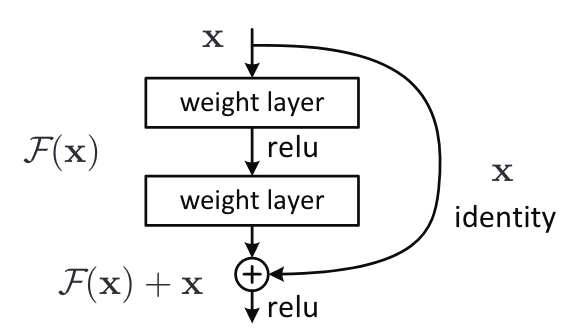
\includegraphics[width=0.6\textwidth]{figures/fig013.png}
    \caption{Fonte: \cite{aiSelfAttentionBasedFusion2023}}
    \label{fig:fig013}
\end{figure}

A ResNet é composta por vários blocos residuais empilhados.
Existem várias versões da \textit{ResNet}, como \textit{ResNet}-18, \textit{ResNet}-34, \textit{ResNet}-50, \textit{ResNet}-101, e \textit{ResNet}-152, onde os números indicam a profundidade total da rede, ou seja, o número de camadas).
% A \textit{ResNet}, desenvolvidas por \cite{heDeepResidualLearning2015}, são arquiteturas convolucionais formada pela composição de blocos residuais, seguidos de uma camada completamente conectada. Estes blocos, ilustrados na Figura 11, empregam o que os autores chamam de \textit{skip connections}, conexões que permitem que camadas sejam puladas durante o treino, resolvendo o problema conhecido como \textit{vanishing gradient}, que afeta principalmente redes neurais profundas e impede o treinamento de progredir por conta de valores muito baixos de gradiente. A inovação trazida por este modelo permitiu a criação de redes muito mais profundas e pode possuir um número definido de camadas, portanto o uso de nomes como ResNet50 ou ResNet101 é uma prática comum para identificar a quantidade de camadas utilizadas no modelo.

%---------------------------------------------------------
\subsection{Features Radiômicas}
\label{subsec:cap4_features_radiomicas}

Serão extraídas características radiômicas de fase diastólica, representada por um conjunto de fatias variando entre 6 e 18 \textit{frames}, de cada paciente usando \gls{GLCM} e estatísticas baseadas em histograma. Será aplicado o filtro \gls{LoG} com cinco valores diferentes em cada parte para suavizar as imagens e realçar as bordas. Foi calculado características \gls{GLCM} como contraste, entropia, correlação, homogeneidade e energia para cada filtro \gls{LoG}. Também é calculado características de intensidade como média, variância, média dos percentis (10 e 90), desvio robusto da média absoluta, curtose e assimetria usando estatísticas de primeira ordem. Foram obtidos 78 características radiômicas para cada paciente dentro da quantidade de fatias extraídas na fase diastólica.

% @TODO - Fase diastólica explicar pag - 33

%---------------------------------------------------------
\subsection{Features Profundas}
\label{subsec:cap4_features_profundas}
 
Para extrair características profundas das imagens de \gls{RMC}, é utilizada a arquitetura pré-treinada de um \textit{ResNet50} sem sua última camada totalmente conectada, treinada no conjunto de dados \textit{ImageNet}. Estudos anteriores demonstraram que o pré-treinamento com \textit{ImageNet} pode melhorar o desempenho de tarefas de classificação de imagens médicas. \textit{ResNet50} é um modelo de rede neural convolucional profunda com 50 camadas que compreende muitos blocos residuais. Cada bloco contém módulos de convolução e uma conexão de salto que transfere a informação do bloco anterior para o próximo bloco. A conexão de salto ajuda a reter a informação semântica mais básica aprendida nas camadas anteriores, que de outra forma se tornaria abstrata devido à conexão de longa cadeia. A conexão de salto também evita o desaparecimento do gradiente nas camadas mais profundas ao fornecer um caminho alternativo para a retropropagação. A informação da conexão de salto é adicionada à informação calculada em cada bloco \cite{aiSelfAttentionBasedFusion2023}. Ao todo são 2048 características coletadas da saída deste modelo.

%---------------------------------------------------------
\subsection{Unificando as Features}
\label{subsec:cap4_unificando_features}

Um vez em posse das features radiômicas, é aplicado um \textit{F-Test} tanto às 78 características radiômicas quanto às 2048 características profundas, reduzindo cada um dos vetores ao espaço de 64 características. No método de fusão convencional, simplesmente é concatenado os dois vetores de características como na Eq. \ref{eq:concat}, onde \textit{Concat} simplesmente concatena os dois vetores. Unificando ambos os vetores obtemos o valor resultante de 128 características o qual será enviado ao mecanismo de autoatenção.

\begin{equation}
F_{hd} = \textit{Concat}(F_h, F_d)
\label{eq:concat}
\end{equation}

%---------------------------------------------------------
\subsection{Módulo de Fusão de Autoatenção}
\label{subsec:cap4_mod_self_attention}

Neste trabalho é empregado o mecanismo de autoatenção para aprender a importância de cada característica e capturar suas dependências de longo alcance. Como ilustrado na Figura \ref{fig:fig011}, o módulo de fusão de autoatenção é utilizado para mapear uma consulta ($Q$), chave ($K$) e valor ($V$) para um valor de atenção. São utilizadas as 128 características concatenadas $F_{hd}$  como \textit{tokens} e projetada cada característica em três matrizes aprendíveis: matriz chave $K$, matriz consulta $Q$ e matriz de valor $V$ por produto escalar com as matrizes $W_{Q}$, $W_{K}$ e $W_{V}$. Logo os valores $Q$, $K$, $V$ são denotados como $W_{Q}F_{gd}$, $W_{K}F_{gd}$, $W_{V}F_{gd}$ respectivamente, onde $W_{Q}$, $W_{K}$ e $W_{V}$ representam a transformação linear para as matrizes $Q$, $K$ e $V$. O módulo de fusão baseado em autoatenção é definido como segue na Equação \ref{eq:attention}, onde $d_{k}$ é a dimensão do valor de $K$. Sem utilizar operações recorrentes ou convolucionais, o módulo de fusão de autoatenção pode modelar as dependências de longo prazo entre as características de entrada.      Este módulo calcula de forma adaptativa os pesos entre as características com base em sua importância e relevância, capturando de forma mais abrangente as associações entre características radiômicas e profundas. Tal processo realça a capacidade expressiva das características fundidas e permite que o modelo foque mais precisamente nas características mais informativas para prever \gls{CH} e reduzir a influência de características irrelevantes na previsão. Além disso, o modelo pode alocar dinamicamente atenção a diferentes amostras de imagens de \gls{RMC}. Essa flexibilidade permite com que o modelo se adapte melhor à representação de características de diferentes amostras, melhorando a precisão e a generalização da previsão.

%---------------------------------------------------------
\subsection{Função de Perda}
\label{subsec:cap4_funcao_perda}

A função de perda utilizada utilizada no modelo é a função de entropia cruzada binária, do termo  \gls{BCE}, que é calculada pela Eq. \ref{eq:bce} onde $\mathcal{L}_{bce}$ denota o \gls{BCE}, $N$ denota o número de imagens de \gls{RMC}, $r$ denota a classe alvo de \gls{CH} e $\hat{r}$ o valor previsto pelo modelo de \gls{CH}, 1 indica indícios de \gls{CH} e 0 sua ausência.

\begin{equation}
\mathcal{L}_{bce} = -\frac{1}{N} \sum_{i=1}^N
(r_i \ln \hat{r}_i + (1 - r_i) \ln (1 - \hat{r}_i))
\label{eq:bce}
\end{equation}

%---------------------------------------------------------
\subsection{Arquitetura Proposta}
\label{subsec:cap4_arquitetura_proposta}

O esquemático da arquitetura proposta pode ser conferida na Figura \ref{fig:fig011}. A imagens de \gls{RMC} são expostas ao seletor de características via \textit{F-test}, as características selecionadas são concatenadas e enviadas ao módulo de fusão de autoatenção, por fim uma camada linear de 128 características precede um camada linear com um único neurônio para a classificação binária.

% @TODO Mover essa parte. pag - 35

\begin{figure}[htbp]
    \centering
    \caption{Arquitetura Proposta}
    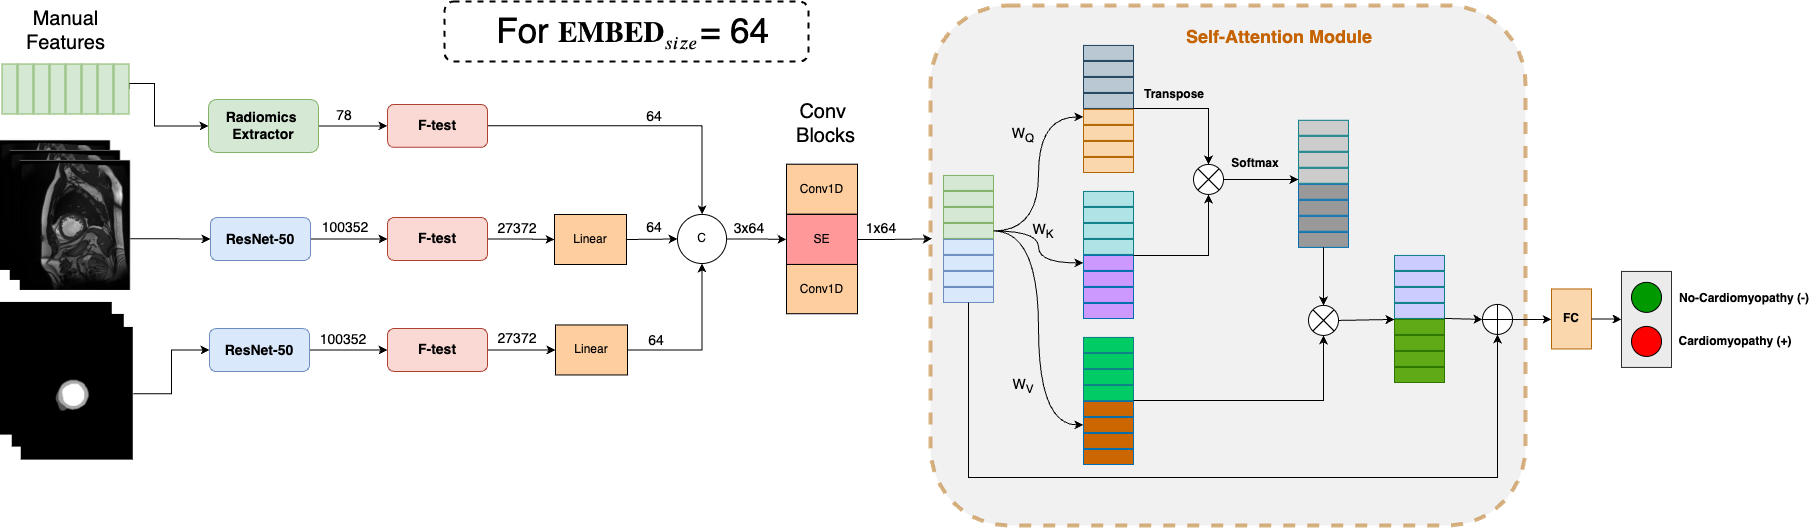
\includegraphics[width=1\textwidth]{figures/fig011.png}
    \caption*{Fonte: Autor}
    \label{fig:fig011}
\end{figure}

Para medir o desempenho da solução serão aplicadas as seguintes métricas: acurácia e precisão, expressas pelas equações \ref{eq:acc}, \ref{eq:precision} e \ref{eq:recall}.
Também é calculada a \gls{AUC}, também reconhecida como a área que avalia o modelo em diversos limites contínuos de decisão, verificando a taxa de verdadeiros positivos contra falsos positivos em cada limite.

% A precisão foi escolhida neste contexto pois quanto maior esta for, menor é a taxa de falso negativo nos resultados. A precisão é pertinente quando o custo com a identificação de falso positivos é alto, como é o caso de doenças fatais.

\begin{equation}
\textit{Acurácia} = \frac{\textit{TP} + \textit{TN}}{\textit{TP} + \textit{TN} + \textit{FP} + \textit{FN}}
\label{eq:acc}
\end{equation}

\begin{equation}
\textit{Precisão} = \frac{\textit{TP}}{\textit{TP} + \textit{FP}}
\label{eq:precision}
\end{equation}

\begin{equation}
\textit{Revocação} = \frac{\textit{TP}}{\textit{TP} + \textit{FN}}
\label{eq:recall}
\end{equation}

%---------------------------------------------------------
% \subsection{Unificando as Features}
% \label{subsec:cap4_unificando_features}

% Um vez em posse das features radiômicas, é aplicado um F-Test e reduz-se cada um dos vetores à 64 características. Unificando ambos os vetores obtemos um vetor de características de tamanho 128 o qual passará pelo mecanismo de \textit{attention}.

%---------------------------------------------------------
\subsection{Fluxograma}
\label{subsec:cap4_floxugrama}

A Figura \ref{fig:fig015} confere o fluxograma do projeto ilustrando de forma esquemática suas fases de atuação.

% @TODO Mover essa parte. pag - 36

\begin{figure}[htbp]
    \centering
    \caption{Fluxograma do Projeto}
    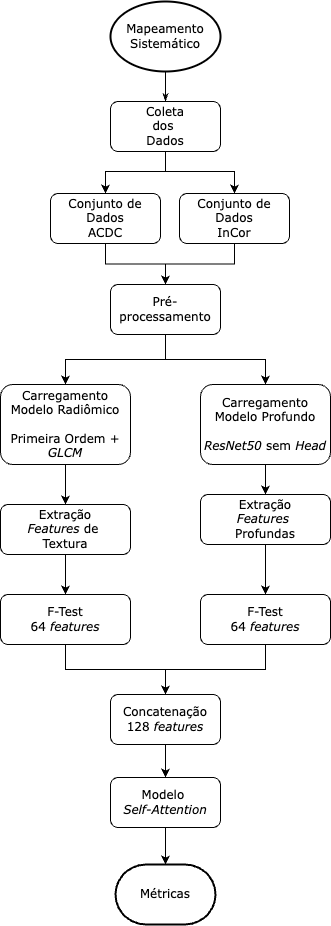
\includegraphics[width=0.4\textwidth]{figures/fig015.png}
    \caption*{Fonte: Autor}
    \label{fig:fig015}
\end{figure}

% @TODO Acrescentar dados Incor e ACDC. pag - 37


%---------------------------------------------------------
\section{Considerações Finais do Capítulo}
\label{sec:cap4_consideracoes_finais}

Como considerações, destacam-se o uso de base de dados pública, com dados de pacientes incluindo o conjuntos de fatias que identificam a ação de sístole e diástole do coração. É aplicado pré-processamento do qual é extraído manualmente 78 características radiômicas, características estas que analisam textura, níveis e variações dos tons de cinza incluindo diversas estatísticas como de primeira ordem e o \gls{GLCM}. Ainda em fase de pré-processamento é extraída as características profundas oriundas do modelo de visão \textit{ResNet50}, com os pesos treinados na base de dados da \textit{ImageNet}. É removida a última camada linear da \textit{ResNet50} resultando ao seu final, sem a camada classificadora, 2048 características. Em posse de ambas as features, é aplicada a técnica de \textit{F-test} para obter as 64 características mais relevantes e, após, concatená-las obtendo um vetor de características de 128 características. Este vetor é exposto ao módulo de fusão com autoatenção, identificando as características mais determinantes independente de espacialidade. 